
% \titlegraphic{\hfill\includegraphics[height=1.5cm]{logo.pdf}}

\documentclass[xcolor=pdftex,dvipsnames,table,numbers,hyperref={pdfpagelabels=false},compress]{beamer}
%\usepackage{requiredPackage}
\usepackage{amsmath}
\usepackage{graphicx}
\usepackage{amsfonts}
\usepackage{amssymb}

\usepackage{tabularx}
\usepackage{epstopdf}
\usepackage{overpic}
\usepackage{url}
\usepackage{calrsfs}
\usepackage{mathrsfs}
\usepackage{epsfig}
\usepackage{cancel}
\usepackage{changepage}

\usepackage{tikz}
\usepackage[customcolors]{hf-tikz} 

\usepackage{lmodern}
%\usepackage{mystyle}
\usepackage{subfig}
\usepackage{pifont}
\usepackage{tabu}
\usepackage{xcolor}
\usepackage{algorithm}
\usepackage{algpseudocode}
%\usepackage{enumitem}
\usepackage{remreset}
\usepackage{etoolbox}
\usepackage{comment} % end and begin comment
%\usepackage{dtklogos} 
\usepackage{listings}
\lstset{breaklines=true} 

\newcommand{\gline}{\textcolor{gray}{\hline}}
\newcommand{\cmark}{\ding{51}}%
\newcommand{\xmark}{\ding{55}}%
\newcommand{\gcheck}{\textcolor{blue}{\Large \cmark}}
\newcommand{\rcross}{\textcolor{red}{\Large \xmark}}
\newcommand{\tkt}{\tilde{K}_\theta}
\newcommand{\kt}{K_\theta}
\newcommand{\ind}{\overset{ind}{\sim}}
\newcommand{\plim}{\overset{p}{\rightarrow}}
\newcommand{\cx}{\frac {X'X}n}
\newcommand{\cz}{\frac {Z'Z}n}
\newcommand{\ccz}{\frac {Z'Z}n - \Sigma_A}
\newcommand{\czy}{\frac {Z'y}n}
\newcommand{\cyz}{\frac {y'Z}n}
\newcommand{\cxy}{\frac {X'y}n}
\newcommand{\cyx}{\frac {y'X}n}
\newcommand{\myitem}{\vskip3mm \item}

\newcommand{\calS}{{\cal S}}
\newcommand{\calA}{{\cal A}}
\newcommand{\calK}{{\cal K}}
\newcommand{\calX}{{\cal X}}
\newcommand{\calD}{{\cal D}}
\newcommand{\calG}{{\cal G}}
\newcommand{\calT}{{\cal T}}
\newcommand{\calU}{{\cal U}}
\newcommand{\calR}{{\cal R}}
\newcommand{\tp}{\tilde{p}}
\newcommand{\tildebC}{\tilde{\bC}}
\newcommand{\calL}{{\cal L}}

\newcommand{\blam}{ \mbox{\boldmath $ \lambda $} }
\newcommand{\bet}{ \mbox{\boldmath $ \eta $} }
\newcommand{\bome}{ \mbox{\boldmath $ \omega $} }
\newcommand{\bbet}{ \mbox{\boldmath $ \beta $} }
\newcommand{\bbeta}{ \mbox{\boldmath $ \beta $} }
\newcommand{\balph}{ \mbox{\boldmath $ \alpha $} }
\newcommand{\balpha}{ \mbox{\boldmath $ \alpha $} }
\newcommand{\bphi}{ \mbox{\boldmath $\phi$}}
\newcommand{\bzeta}{ \mbox{\boldmath $\zeta$}}
\newcommand{\bkap}{ \mbox{\boldmath $\kappa$}}
\newcommand{\bkappa}{ \mbox{\boldmath $\kappa$}}
\newcommand{\beps}{ \mbox{\boldmath $\epsilon$}}
\newcommand{\bepsilon}{ \mbox{\boldmath $\epsilon$}}
\newcommand{\bthet}{ \mbox{\boldmath $ \theta $} }
\newcommand{\btheta}{ \mbox{\boldmath $ \theta $} }
\newcommand{\blambda}{ \mbox{\boldmath $ \lambda $} }
\newcommand{\bnu}{ \mbox{\boldmath $\nu$} }
\newcommand{\bmu}{ \mbox{\boldmath $\mu$} }
\newcommand{\bGam}{ \mbox{\boldmath $\Gamma$} }
\newcommand{\bSig}{ \mbox{\boldmath $\Sigma$} }
\newcommand{\bSigma}{ \mbox{\boldmath $\Sigma$} }
\newcommand{\bPhi}{ \mbox{\boldmath $\Phi$} }
\newcommand{\bThet}{ \mbox{\boldmath $\Theta$} }
\newcommand{\bTheta}{ \mbox{\boldmath $\Theta$} }
\newcommand{\bDel}{ \mbox{\boldmath $\Delta$} }
\newcommand{\bDelta}{ \mbox{\boldmath $\Delta$} }
\newcommand{\bnabla}{ \mbox{\boldmath $\nabla$} }
\newcommand{\bLam}{ \mbox{\boldmath $\Lambda$} }
\newcommand{\bLambda}{ \mbox{\boldmath $\Lambda$} }
\newcommand{\bgam}{ \mbox{\boldmath $\gamma$} }
\newcommand{\bgamma}{ \mbox{\boldmath $\gamma$} }
\newcommand{\brho}{ \mbox{\boldmath $\rho$} }
\newcommand{\bdel}{ \mbox{\boldmath $\delta$} }
\newcommand{\bdelta}{ \mbox{\boldmath $\delta$} }
\newcommand{\sis}{\sigma^2}
\newcommand{\bOmega}{\mbox{\boldmath $\Omega$} }
\newcommand{\bPsi}{ {\boldsymbol \Psi} }
\newcommand{\btkt}{\boldsymbol{\tilde{K}}_\theta}
\newcommand{\pg}{P{\'o}lya-Gamma }

\newcommand{\bzero}{\textbf{0}}
\newcommand{\bones}{\textbf{1}}
\newcommand{\ba}{\textbf{a}}
\newcommand{\bb}{\textbf{b}}
\newcommand{\bB}{\textbf{B}}
%\newcommand{\bA}{\textbf{A}}
\newcommand{\bc}{\textbf{c}}
\newcommand{\bC}{\textbf{C}}
\newcommand{\bA}{\textbf{A}}
\newcommand{\bd}{\textbf{d}}
\newcommand{\bD}{\textbf{D}}
\newcommand{\be}{\textbf{e}}
\newcommand{\bE}{\textbf{E}}
\newcommand{\bk}{\textbf{k}}
\newcommand{\bK}{\textbf{K}}
\newcommand{\bh}{\textbf{h}}
\newcommand{\bs}{\textbf{s}}
\newcommand{\bS}{\textbf{S}}
\newcommand{\bH}{\textbf{H}}
\newcommand{\bI}{\textbf{I}}
\newcommand{\bt}{\textbf{t}}
\newcommand{\bu}{\textbf{u}}
\newcommand{\bv}{\textbf{v}}
\newcommand{\bw}{\textbf{w}}
\newcommand{\bW}{\textbf{W}}
\newcommand{\bx}{\textbf{x}}
\newcommand{\bX}{\textbf{X}}
\newcommand{\by}{\textbf{y}}
\newcommand{\bY}{\textbf{Y}}
\newcommand{\bz}{\textbf{z}}
\newcommand{\bZ}{\textbf{Z}}
\newcommand{\bL}{\textbf{L}}
\newcommand{\br}{\textbf{r}}
\newcommand{\bR}{\textbf{R}}
\newcommand{\bm}{\textbf{m}}
\newcommand{\bM}{\textbf{M}}
\newcommand{\given}{\,|\,}
\newcommand{\T}{\top}
\newcommand{\bV}{\textbf{V}}
\newcommand{\bJ}{\textbf{J}}
\newcommand{\blue}[1]{{\color{RoyalBlue!90} #1}}
\newcommand{\red}[1]{{\color{Red} #1}}
\newcommand{\green}[1]{{\color{Green} #1}}
\newcommand{\orange}[1]{{\color{Orange} #1}}
\newcommand{\titl}[1]{{\begin{large}\begin{center}#1\end{center}\end{large}}}

\newcommand{\tildea}{\tilde{a}}
\newcommand{\tildeba}{\tilde{\ba}}
\newcommand{\tildebv}{\tilde{\bv}}
\newcommand{\tildev}{\tilde{v}}
\newcommand{\tildeA}{\tilde{A}}
\newcommand{\tildeC}{\tilde{C}}
\newcommand{\tildeK}{\tilde{K}}
\newcommand{\tildew}{\tilde{w}}
\newcommand{\tildeu}{\tilde{u}}
\newcommand{\tildebw}{\tilde{\bw}}
\newcommand{\tildeeps}{\tilde{\epsilon}}
\newcommand{\tildebeps}{\tilde{\bepsilon}}
\newcommand{\eps}{\epsilon}
\newcommand{\sigs}{\sigma^2}
\newcommand{\taus}{\tau^2}
\newcommand{\iid}{\stackrel{\mathrm{iid}}{\sim}}

%\newcommand{\calS}{{\cal S}}
\newcommand{\calC}{{\cal C}}

%\documentclass[10pt]{beamer}

\usetheme{metropolis}
\usepackage{appendixnumberbeamer}

\usepackage{booktabs}
\usepackage[scale=2]{ccicons}

\usepackage{pgfplots}
\usepgfplotslibrary{dateplot}

\usepackage{xspace}
\newcommand{\themename}{\textbf{\textsc{metropolis}}\xspace}

\makeatletter
\@addtoreset{subfigure}{framenumber}% subfigure counter resets every frame
\makeatother

\makeatletter
\@addtoreset{figure}{framenumber}% subfigure counter resets every frame
\makeatother

\setbeamertemplate{caption}{\raggedright\insertcaption\par}
\captionsetup[subfigure]{labelformat=empty}


\title[]{Conjugate Bayesian Models for Massive Spatial Data}
\author{Andrew Finley$^1$ \& Jeffrey Doser$^2$}
	
\institute{
\begin{tiny}$^1$Department of Forestry, Michigan State University.\\
$^2$Department of Integrative Biology, Michigan State University.\end{tiny}
}

\date{May 15, 2023}


\begin{document}

\maketitle
\begin{frame}{Case Study: Alaska Tanana Valley Forest Height Dataset}
	\vskip -5mm \begin{figure}[!ht]
		\begin{center}
			\subfloat[Forest height and tree cover]{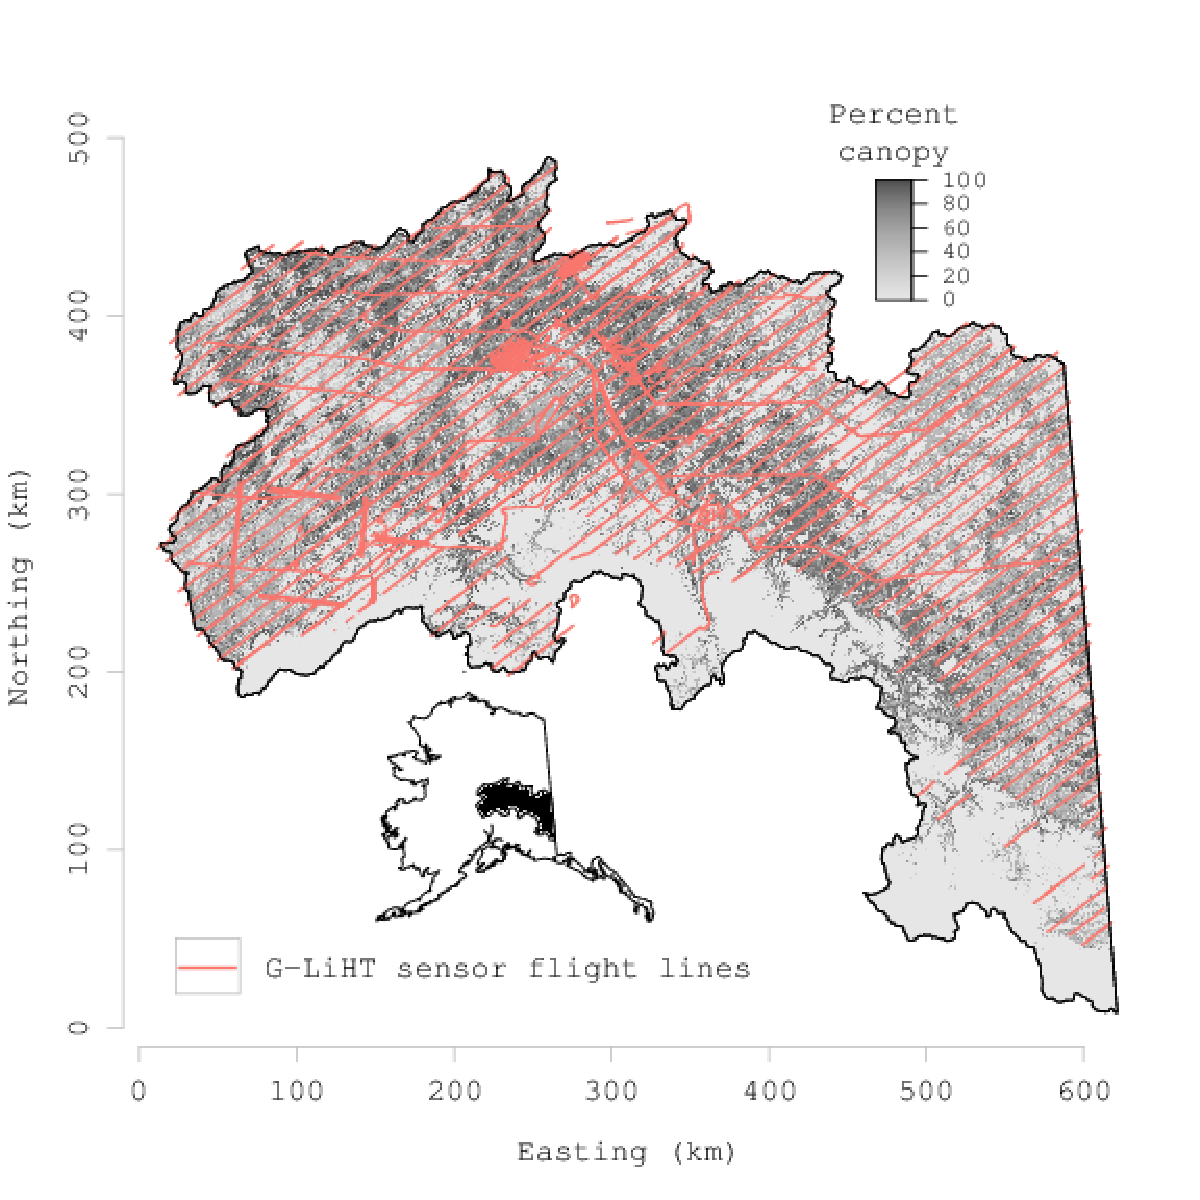
\includegraphics[width=5.3cm]{../figures/ak-flight-han2010.pdf}\label{han}}
			\subfloat[Forest fire history]{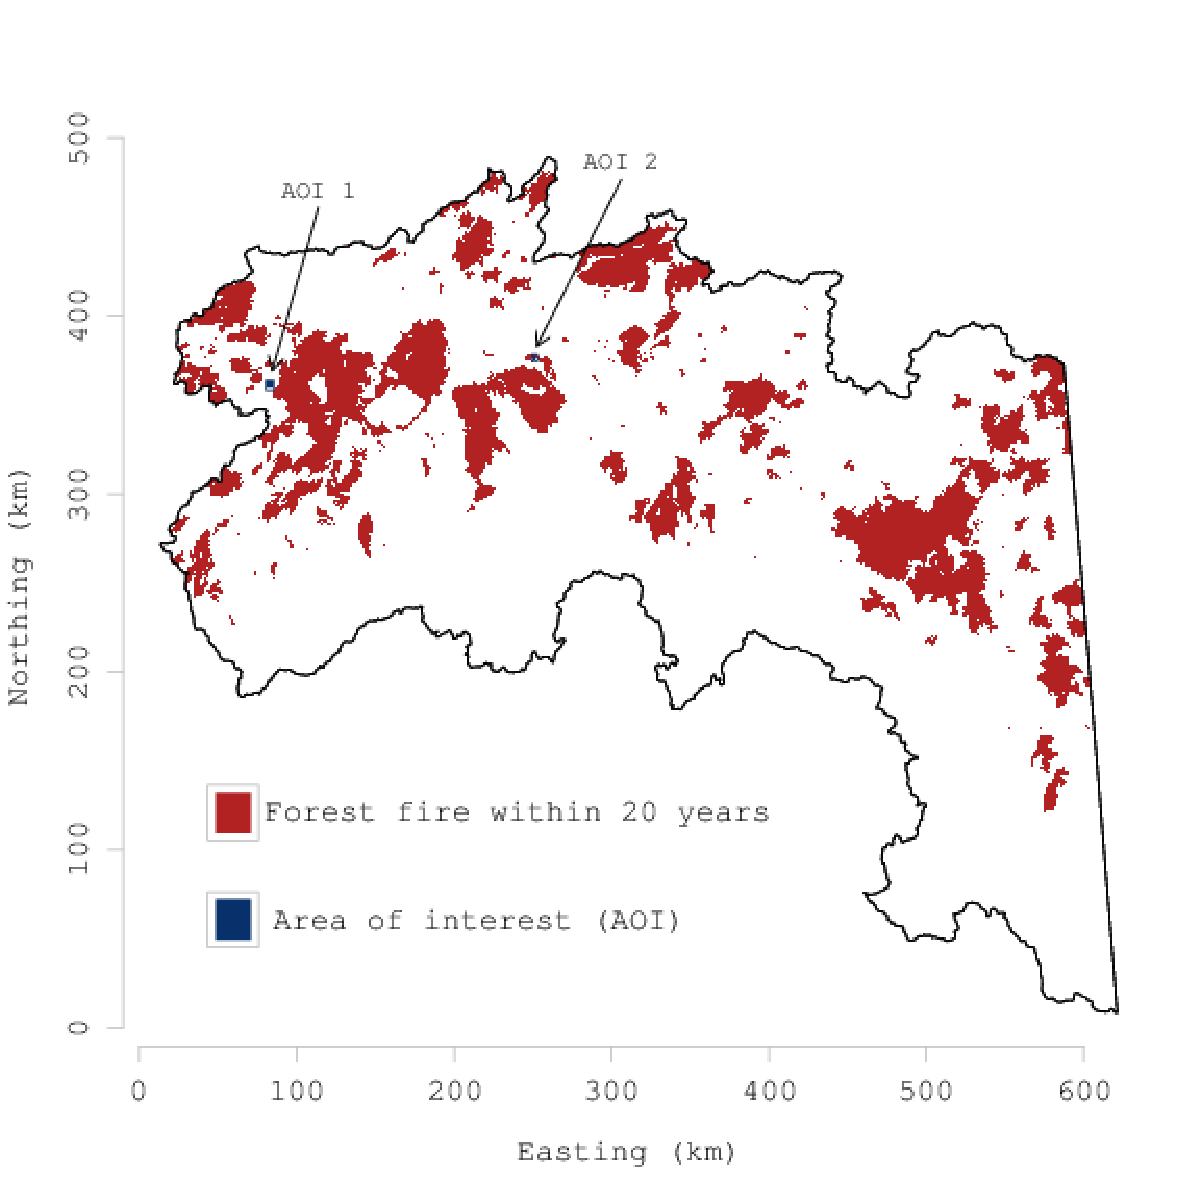
\includegraphics[width=5.3cm]{../figures/ak-fire.pdf}\label{fire}}
		\end{center}
		%\caption{Tanana valley, Alaska, study region. \subref{han} G-LiHT flight lines where canopy height was measured at 6x$10^6$n locations over the percent forest canopy covariate. \subref{fire} Occurrence of forest fire in the past 20 years and areas of interest for prediction illustration.}
	\end{figure}
	\vskip -4mm 
	\only<1>{\begin{itemize}
			\item Forest height (red lines) data from LiDAR at \red{$5\times 10^6$} locations
			\item Knowledge of forest height is important for biomass assessment, carbon management etc
	\end{itemize}}
	\only<2>{\begin{itemize}
			\item Goal: High-resolution domainwide prediction maps of forest height 
			 \item Covariates: Domainwide tree cover (grey) and forest fire history (red patches) in the last 20 years 
			%\item Goal: Domainwide prediction of forest height 
	\end{itemize}}
\end{frame}

\begin{frame}{Analyzing the data}
	Models used:
	\begin{itemize}
		\item Non-spatial regression: $y_{FH}(s) = \beta_0 + \beta_{tree} x_{tree} + \beta_{fire} x_{fire} + \eps(s)$
	\end{itemize}
	
	\begin{figure}
		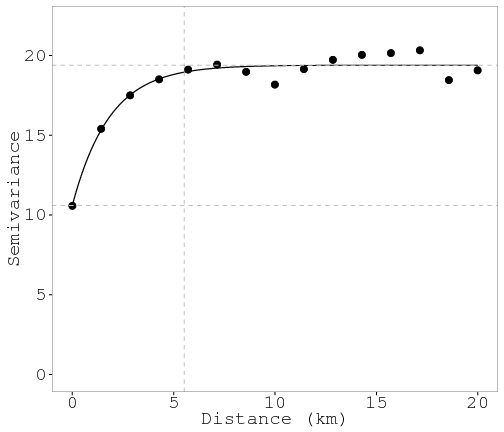
\includegraphics[scale=0.25]{../figures/non-sp-resid-variog.png}
	\caption{Variogram of the residuals from non-spatial regression indicates \red{strong spatial pattern}}
	\end{figure}

\end{frame}

\begin{frame}{NNGP models}
\begin{itemize}
		\item Collapsed NNGP: 
		\begin{itemize}
			\item $y_{FH}(s) = \beta_0 + \beta_{tree} x_{tree} + \beta_{fire} x_{fire} + w(s)+ \eps(s)$
			\myitem $w(s) \sim NNGP(0,C(\cdot,\cdot \given \sigs, \phi))$
			\myitem $y_{FH} \sim N(X\beta, \tilde C + \taus I)$ where $\tilde C$ is the NNGP covariance matrix derived from $C$
		\end{itemize}
		
		\myitem Response NNGP: 
		\begin{itemize}
		\item $y_{FH}(s) \sim NNGP( \beta_0 + \beta_{tree} x_{tree} + \beta_{fire} x_{fire}, \Sigma(\cdot, \cdot \given \sigs, \phi, \taus)) $
		\myitem $y_{FH} \sim N(X\beta, \tilde \Sigma)$ where $\tilde \Sigma$ is the NNGP covariance matrix derived from $\Sigma = C + \taus I$
		\end{itemize}
	
\end{itemize}
\end{frame}
	
\begin{frame}{NNGP models}
\begin{table}
{\small	\begin{tabular}{cccc}
& 		Non-spatial regression & Collapsed NNGP & Response NNGP \\ \hline
CRPS & 2.3 & 0.86 & 0.86 \\
RMSPE & 4.2 & 1.73 & 1.72 \\
CP & 93\% & 94\% & 94\% \\
CIW & 16.3 & 6.6 & 6.6 \\\hline
	\end{tabular}}
\caption{Model comparison metrics for the Tanana valley dataset}
\end{table}
\vskip -4mm \begin{itemize}
	\item NNGP models perform significantly better than the non-spatial model
	\item MCMC run time for the NNGP models:
		\begin{itemize}
			\item Collapsed model: \red{$319$} hours
			\item Response model: \red{$38$} hours
		\end{itemize}
	\item For \red{massive} spatial data, full Bayesian output for even NNGP models require substantial time
\end{itemize}
\end{frame}

\begin{frame}{Another look at the response model}
	\begin{itemize}
	\item Original full GP model: $y(s) \ind N(x(s)'\beta + w(s), \taus)$
	\item $w(s) \sim GP$ with a stationary covariance function $C(\cdot, \cdot \given \sigs, \phi)$  
	\item $Cov(w) = \sigs R(\phi)$
	\item Full GP model: $y \sim N(X\beta, \Sigma)$ where $\Sigma = \sigs M$
	\item $M= R(\phi) + \alpha I$
	\item $\alpha = \taus/\sigs$ is the ratio of the \alert{noise to signal variance}
	\item Response NNGP model: $y \sim N(X\beta, \tilde \Sigma)$
	\item $\tilde \Sigma = \sigs \tilde M$ where $\tilde M$ is the NNGP approximation for $M$
	\end{itemize}
\end{frame}

\begin{frame}{Conjugate NNGP}
\begin{itemize}
\item $y \sim N(X\beta, \sigs \tilde M)$
\item If $\phi$ and $\alpha$ are known, $M$, and hence $\tilde M$, are known matrices
\item The model becomes a standard Bayesian linear model
\item Assume a \alert{\em Normal Inverse Gamma (NIG)} prior for $(\beta, \sigs)'$
\item $(\beta, \sigs)' \sim NIG(\mu_\beta, V_\beta, a_\sigma, b_\sigma)$, i.e., $\beta \given \sigs \sim N(\mu_\beta, \sigs V_\beta)$ and $\sigs \sim IG(a_\sigma, b_\sigma)$
\end{itemize}
\end{frame}

\begin{frame}{Conjugate NNGP}
\begin{itemize}
\item $y \sim N(X\beta, \sigs \tilde M)$, $\tilde M$ is known
\vskip 5mm 
{\metroset{block=fill}
\begin{alertblock}{Joint likelihood:}
\[N(y \given X\beta, \sigs \tilde M) \times N(\beta \given \mu_\beta, \sigs V_\beta) \times IG(\sigs \given a_\sigma, b_\sigma) \]
\end{alertblock}}
\pause
\myitem \red{Conjugate posterior distribution} $(\beta, \sigs) \given y \sim NIG(\mu_\beta^*, V_\beta^*, a_\sigma^*, b_\sigma^*)$
\myitem Expressions for $\mu_\beta^*$, $V_\beta^*$, $a_\sigma^*$ and $b_\sigma^*$ can be calculated in \red{$O(n)$} time
\end{itemize}
\end{frame}

\begin{frame}{Conjugate NNGP}
\begin{itemize}
\item $(\beta, \sigs) \given y \sim NIG(\mu_\beta^*, V_\beta^*, a_\sigma^*, b_\sigma^*)$
\item \red{Marginal posterior:} $\beta \given y \sim MVt_{2a_\sigma^*}(\mu_\beta^*, \frac {b_\sigma^*}{a_\sigma^*} V_\beta^*)$
\item $MVt_k(m,V)$ is the \alert{\em multivariate $t$} distribution with degrees of $k$, mean $m$ and scale matrix $V$
\item $E(\beta \given y) = \mu_\beta^*$, $Var(\beta \given y) = \frac{b_\sigma^*}{a_\sigma^*{-1}} V_\beta^*$
\item \red{Marginal posterior:} $\sigs \given y \sim IG(a_\sigma^*, b_\sigma^*)$
\item $E(\sigs \given y) = \frac{b_\sigma^*}{a_\sigma^*-1}$, $Var(\sigs \given y) = \frac{b_{\sigma}^{*2}}{(a_\sigma^*-1)^2(a_\sigma^*-2)}$
\item \green{Exact posterior distributions} of $\beta$ and $\sigs$ are available
\end{itemize}
\end{frame}

\begin{frame}{Predictive distributions}
\begin{itemize}
\item $y(s) \given y \sim t_{2a_\sigma^*}{(m(s) , \frac{b_\sigma^*}{a_\sigma^*} v(s)})$
\myitem $E(y(s) \given y) = m(s)$, $Var(y(s) \given y) = \frac{b_\sigma^*}{a_\sigma^*{-1}} v(s)$
\myitem $m(s)$ and $v(s)$ can be computed using \red{$O(m)$} flops
\myitem \green{Exact posterior predictive distributions} of $y(s) \given y$ for any $s$
%\item \green{Exact posterior distributions} of $\beta$ and $\sigs$ and \blue{predictive posterior distributions} of $y(s_0) \given y$ available
\myitem \red{No MCMC} required for parameter estimation or prediction
%\item $\mu_\beta^*$, $V_\beta^*$, $a_\sigma^*$, $ b_\sigma^*$  , 
%\item \red{Available} in the spNNGP package
\end{itemize}
\end{frame}

\begin{frame}{Choosing $\alpha$ and $\phi$}
\begin{itemize}
\item $\phi$ and $\alpha$ are chosen using $K$-fold \alert{cross validation} over a grid of possible values
\item Unlike MCMC, cross-validation can be \red{completely parallelized}
\item Resolution of the grid for $\phi$ and $\alpha$ can be decided based on computing resources available 
\item In practice, a reasonably coarse grid often suffices 
\end{itemize}
\end{frame}

\begin{frame}{Choosing $\alpha$ and $\phi$}
\begin{figure}[!ht]
\begin{center}
	\subfloat[RMSPE]{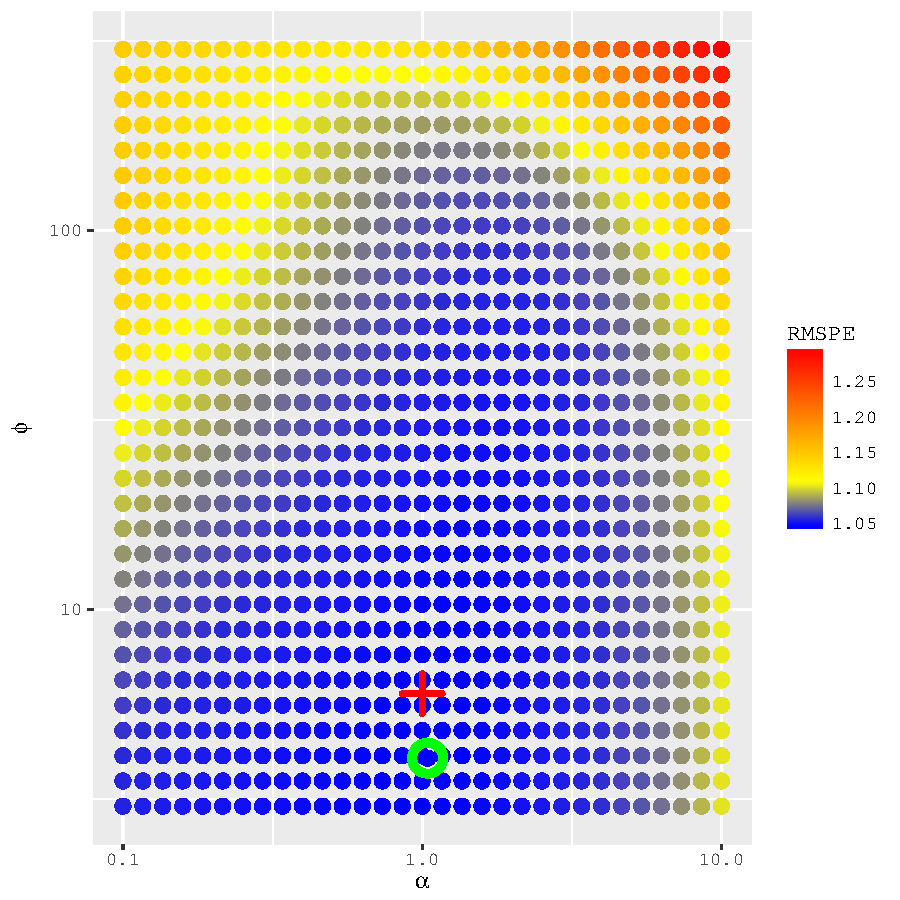
\includegraphics[scale=0.35]{../figures/n50k-m15-reg-rmspe.pdf}\label{syn-xval-rmspe}}
\end{center}
\caption{Simulation experiment: True value (\red{$+$}) of $(\alpha,\phi)$ and estimated value ({\color{green} $\circ$}) using 5-fold cross validation }
\end{figure}
\end{frame}

\begin{frame}{Scalability}
\begin{itemize}
\item Computation and storage requirements are \red{$O(n)$}
\item One evaluation time similar to the response NNGP model
\item Unlike response NNGP, does not involve any serial MCMC iterations
\item For $K$ fold cross validation and $G$ combinations of $\phi$ and $\alpha$, total number of evaluations is $KG$
\item \alert{Embarassingly parallel:} Each of the $KG$ evaluations can proceed in parallel
\end{itemize}
\end{frame}

\begin{frame}{Scalability}
\begin{figure}
\center
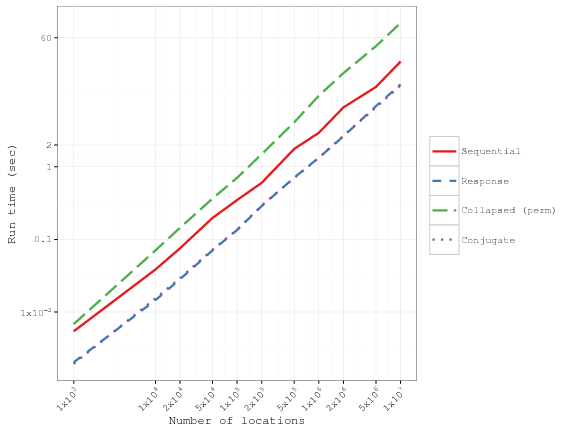
\includegraphics[scale=0.45]{../figures/model-n-vs-time.png}
\caption{Run times of different NNGP models with increasing sample size}
\end{figure}
\end{frame}

\begin{frame}{Alaska Tanana Valley dataset}
\begin{table}
\begin{adjustwidth}{-10mm}{-15mm}
\begin{center}
{\small	\begin{tabular}{cccc}
& 		\red{Conjugate NNGP} & Collapsed NNGP & Response NNGP \\ \hline
$\beta_0$  &\red{2.51}&2.41 (2.35, 2.47)&2.37 (2.31,2.42)\\
$\beta_{TC}$  &\red{0.02}&0.02 (0.02, 0.02)&0.02 (0.02, 0.02)\\
$\beta_{Fire}$  &\red{0.35}&0.39 (0.34, 0.43)&0.43 (0.39, 0.48)\\
$\sigma^2$  &\red{23.21}&18.67 (18.50, 18.81)&17.29 (17.13, 17.41)\\
$\tau^2$  &\red{1.21}&1.56 (1.55, 1.56)&1.55 (1.54, 1.55)\\
$\phi$  &\red{3.83} &3.73 (3.70, 3.77) & 4.15 (4.13, 4.19)\\
CRPS & \red{0.84} & 0.86 & 0.86 \\
RMSPE & \red{1.71} & 1.73 & 1.72 \\
\rowcolor{yellow} time (hrs.) & \red{0.002} & 319 & 38 \\ \hline
	\end{tabular}}
\end{center}
\end{adjustwidth}
\caption{Parameter estimates and model comparison metrics for the Tanana valley dataset}
\end{table}
\vskip -5mm \begin{itemize}
\item Conjugate model produces estimates and model comparison numbers very similar to the MCMC based NNGP models
\item For \red{$5\times10^6$} locations, conjugate model takes \red{$7$ seconds}
\end{itemize}
\end{frame}

\begin{frame}{Summary}
\begin{itemize}
\item \red{MCMC free} exact Bayesian approach by fixing some covariance parameters
\item Conjugate posterior distributions of the parameters and   posterior predictive distributions available in closed form 
\item \blue{Embarassingly parallel} cross validation to identify best choices for fixed parameters
\item Runs in \green{seconds} for massive spatial dataset with \red{millions} of locations
\item Available in the \blue{spNNGP} package in R
\end{itemize}
\end{frame}

\end{document}
